\nonstopmode
\documentclass[ignorenonframetext]{beamer}

\usepackage{graphicx}
\usepackage{url}
\usepackage{textcomp}
\usepackage{listings}
\usepackage{amsmath,amssymb,amsfonts,amsthm,esint}
\newcommand{\abbr}[1]{#1}

\renewcommand{\mit}{\abbr{MIT}}

\newcommand{\latexinput}[1]{\lstset{language=[LaTeX]TeX}\lstinputlisting{#1}}

\usetheme{CambridgeUS}
\setcounter{tocdepth}{1}

\title{Introduction to \LaTeX}
\author[Benjamin Barenblat]{Benjamin Barenblat\\\url{bbaren@mit.edu}}
\institute[\abbr{SIPB}/\mit]{%\includegraphics[height=0.6in]{images/fuzzball.pdf}\\
  Student Information Processing Board\\Massachusetts Institute of Technology}
\date{January 12, 2011}

\begin{document}
\maketitle

Hi, and welcome to Introduction to \LaTeX.  My name is Benjamin
Barenblat; I'm a current undergraduate here at \mit, and my goal
tonight is to reduce the learning curve that is generally associated
with one of the finest computer typesetting packages -- indeed,
probably one of the finest pieces of computer software -- in existence
today.

Before we go any further, I'd like to briefly thank the Student
Information Processing Board of \mit, specifically Andrew
Farrell, for arranging for me to have this room and for publicizing
the class.  Thanks.

\begin{frame}
  \titlepage
\end{frame}

\section*{Outline}
So as I mentioned, my primary goal tonight is to reduce a learning
curve.  \LaTeX\ is a fantastically powerful piece of software, but it
can be daunting just getting started.  So tonight, I'm going to make
every effort to present without expecting prior knowledge about
\LaTeX, \TeX, or even programming in general.  If you have this
knowledge, hopefully I'll do a good job connecting it to some things
you may not have learned before, and hopefully, you'll understand even
better.  But for those who have never programmed, we'll start at
square one.  \LaTeX\ really is a programming language, and
understanding it as such will help you prepare documents.  However, I
wouldn't be a very good teacher if I didn't give you tools to further
your own education, so my goal here is really twofold: first, to
reduce the \LaTeX\ learning curve, and second, to teach you how to get
help with \LaTeX, both here at \mit\ and in other settings as well.

First, though, we'll start out with some \LaTeX\ history and
philosophy; I'll then guide you through the basic procedures inherent
in document preparation.  We'll look at some sample documents and
examine some core language features, so hopefully, by the end of the
hour, you should be able to produce relatively sophisticated
\LaTeX\ documents suitable for, say, a humanities paper.  In the
second hour, we'll look at how \LaTeX\ handles one of its strongest
suits -- mathematics -- as well as how it can serve as a replacement
for Microsoft PowerPoint.  (This presentation was prepared entirely in
\LaTeX.)  We'll also spend a little time discussing how to install
\LaTeX\ on your own machine, and then we'll hopefully have time for
questions.  However, feel free to interrupt at any time.  Also, these
slides will be available online, so don't worry about frantically
scribbling notes while I blaze through.

\begin{frame}
  \tableofcontents
\end{frame}


\section{Introduction} 
% History lesson, goals, etc.--15 min.
\subsection{What is \LaTeX?}
To really understand what \LaTeX\ is and how it should be used, we
have to step in the Way Back Machine and set the dials for 1962, when
a computer scientist named Donald Knuth started writing a book on
compiler design.

\begin{frame}
  \begin{figure}
    \centering
    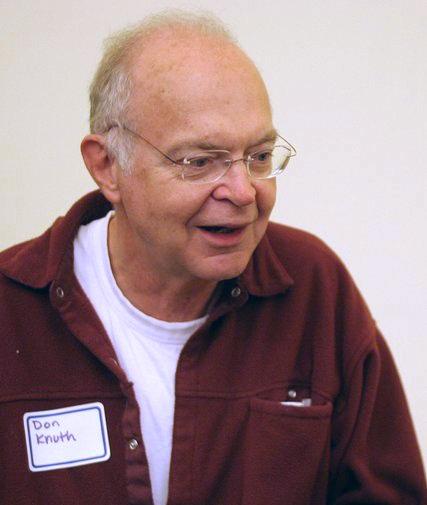
\includegraphics[height=3in]{images/knuth.jpg}
    \caption{Donald Knuth in 2005.  \emph{Source: Wikimedia Commons.}}
    \label{fig:knuth}
  \end{figure}
\end{frame}

Back in the '60s, when you wrote a book, you \emph{wrote} a book, so
Knuth, aiming for a 600-page book, estimated that five written pages
would translate to one typeset page and wrapped up his remarks right
around 3,000 handwritten pages.  As it turns out, though, it only
takes about 1\textonehalf\ handwritten pages to produce a typeset
page, which put Knuth's book at 2,000 pages.  Clearly, he had far more
to say than could fit in a book on compiler design -- indeed, more
than could fit in a single volume.  So Knuth's book on compiler design
turned into a monograph, \emph{The Art of Computer Programming.}

\begin{frame}
  \begin{figure}
    \centering
    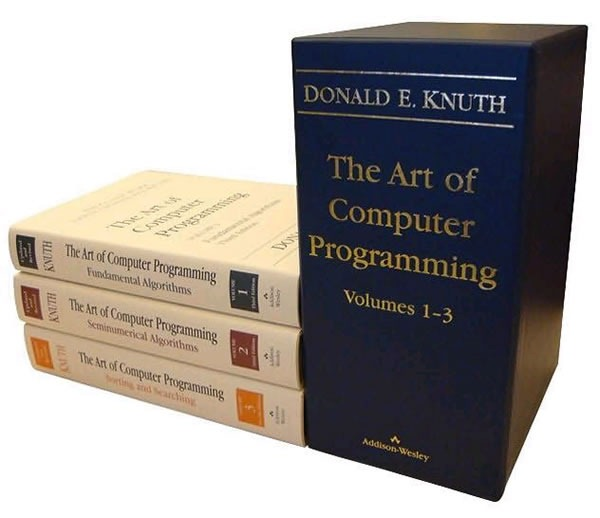
\includegraphics[width=2.25in]{images/aocp.jpg}
    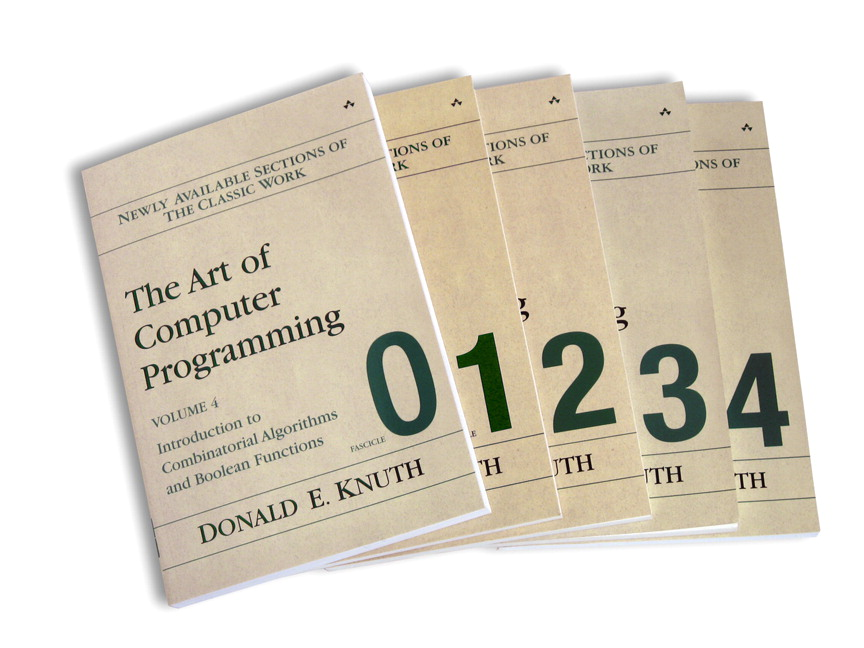
\includegraphics[width=2.25in]{images/aocp-vol2.jpg}
    \caption{\emph{The Art of Computer Programming.} \emph{Source: \abbr{MSDN}.}}
    \label{fig:aocp}
  \end{figure}
\end{frame}

It's now up to four massive volumes -- he hasn't finished it yet --
and has been acknowledged as one of the seminal monographs of the 20th
century.  Volume 1 was printed in 1969, and Knuth finished volume 2 in
1976.  By this point Knuth's publisher was looking into a second
edition of the first volume, so the publisher reset the type for the
first volume, typeset the second volume, and sent proofs of both to
Knuth.

However, when Knuth received the proofs, they looked awful -- the new
edition of volume 1 looked nothing like the old.  Knuth called the
publisher and asked what had happened; the publisher told him that
during the early '70s, they had switched to computer typesetting and
that his proofs were the ones the computer produced.  Knuth, however,
realized that the computer typesetting program produced ugly output,
so he did what any self-respecting computer scientist would do: he
wrote his own.  He took a sabbatical, and in 1978, he started writing
his typesetter.  However, one thing led to another, and Knuth's
typesetter finally saw official release in 1989, eleven years later.
It was written entirely in a literate programming style and included a
specialized Turing-complete typesetting language.  Knuth called it
\TeX.

\begin{frame}
  \begin{figure}
    \centering
    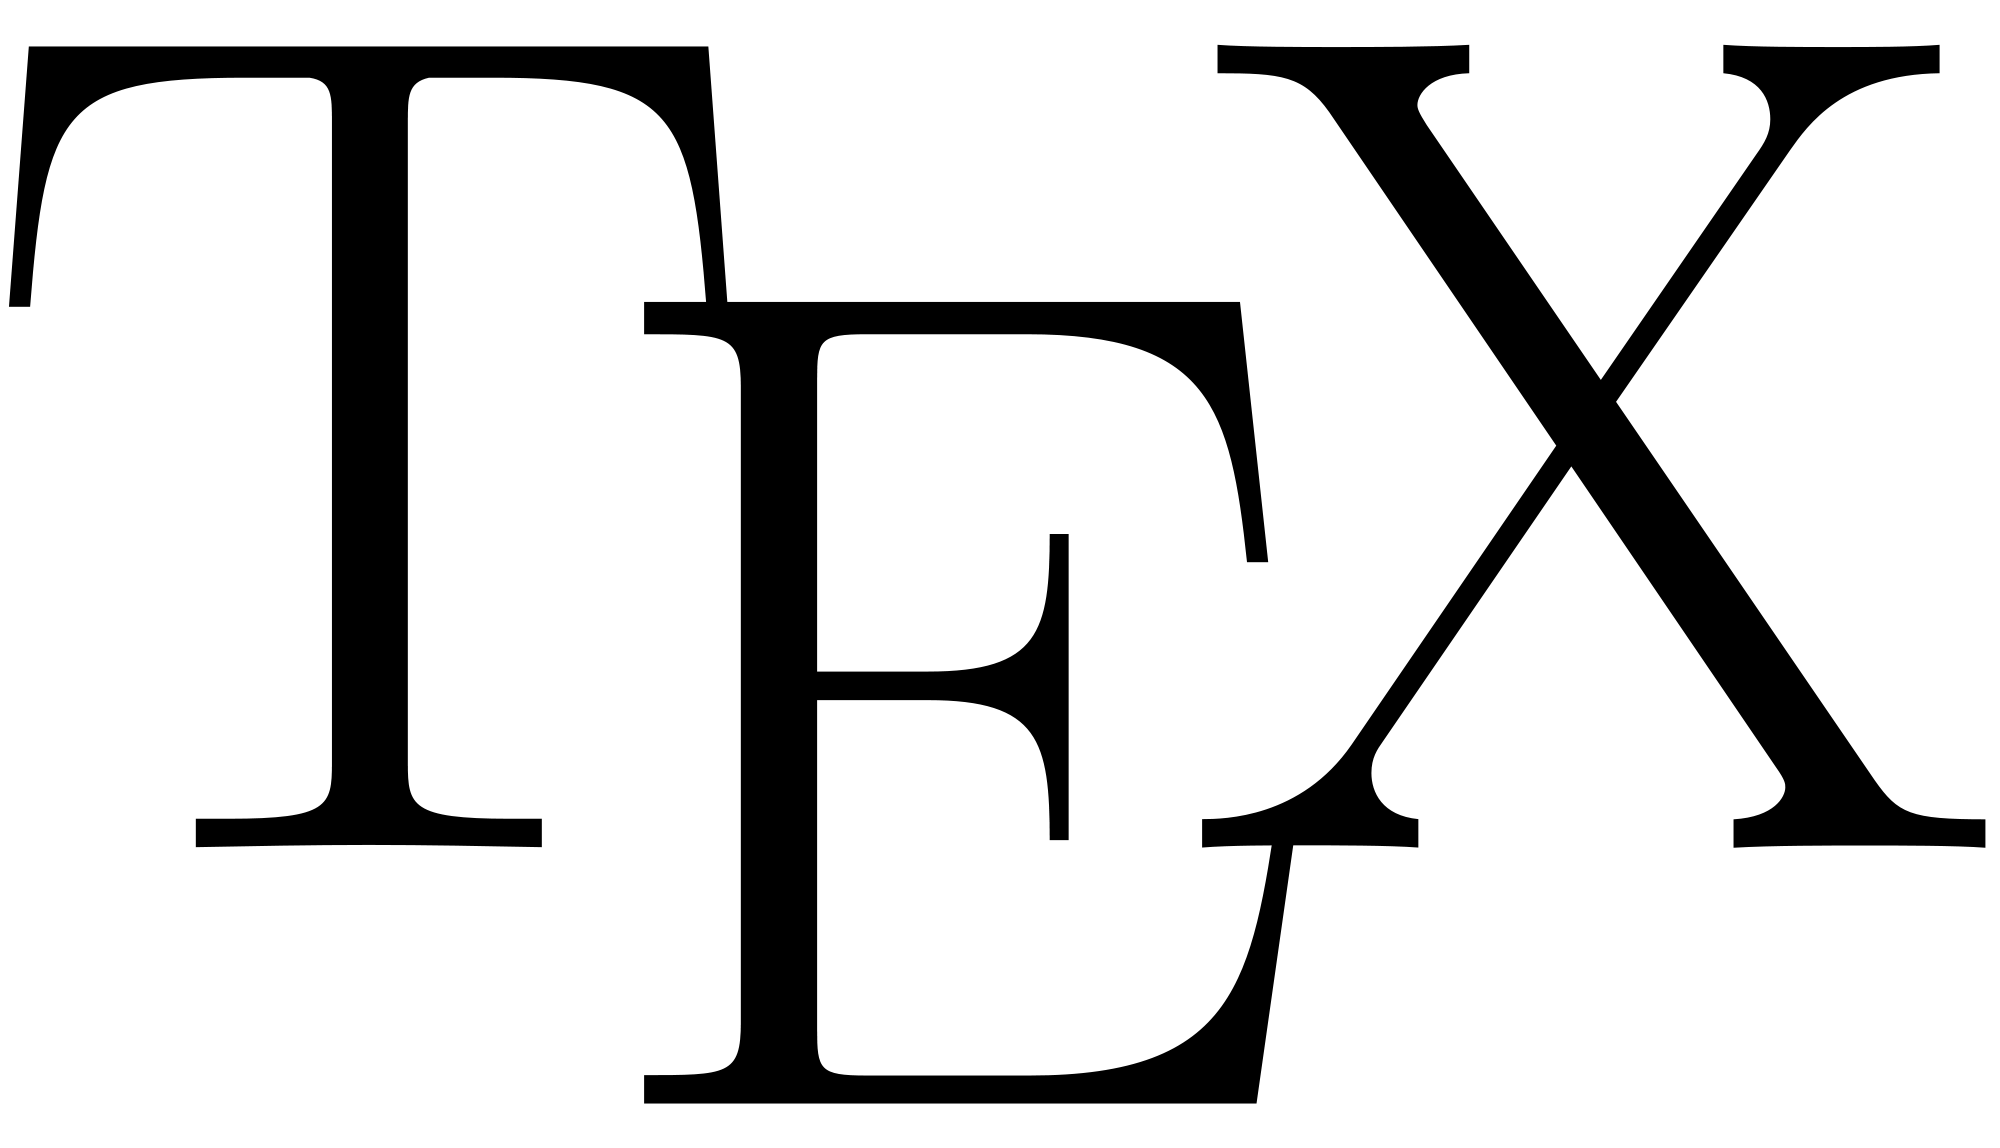
\includegraphics[width=4.5in]{images/tex.png}
    \caption{The \TeX\ logo.}
    \label{fig:texlogo}
  \end{figure}
\end{frame}

\TeX\ took the scientific world by storm, primarily because Knuth had
devoted a siginficant portion of his eleven years to learning how to
typeset mathematics.  The result was that \TeX, unlike any other
typesetting program of the day, could accept mathematical formulas as
input and produce beautiful, readable output.  Nobody had seen
anything like it.

\begin{frame}
  \begin{figure}
    \centering
    \lstset{language=TeX}
   \scriptsize
    \lstinputlisting{code/math.tex}
 \caption{Some \TeX\ code.  \emph{Source: The Lone \TeX{}nician.}}
    \label{fig:texcode}
  \end{figure}
\end{frame}

Nobody could figure out how to use it, either.  \TeX\ is an incredibly
complicated language, and it requires you to micromanage every aspect
of your document.  You have to explicitly specify which text should
appear bold, which italic, where paragraph and page breaks should be,
and so on.  If you want a section heading, you have to tell \TeX\ to
make your text bold 18-point every single time.  Incidentally, this is
the model generally followed by users of another program: Microsoft
Word.  \TeX\ is effectively Microsoft Word on steroids, and it's a
pain to use.  Nobody would use it to write a paper, much less an
entire book!

At least, that's what was going through the head of Leslie Lamport in
the early '80s as he was writing the Great American Concurrency Book.

\begin{frame}
  \begin{figure}
    \centering
    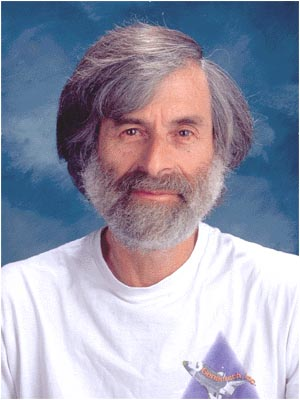
\includegraphics[height=3in]{images/lamport.jpg}
    \caption{Leslie Lamport in 2004.  \emph{Source: Wikimedia Commons.}}
    \label{fig:lamport}
  \end{figure}
\end{frame}

Sick and tired of telling \TeX\ to make text 18-point bold over and
over and over again, Lamport did what any self-respecting computer
scientist would do: he started making use of that Turing-complete
language embedded in \TeX, and he started writing new commands for
\TeX\ that would make it set section headers in 18-point bold
automatically.  So instead of telling \TeX\ to make text 18-point
bold, Lamport would just tell \TeX\ that the text was a section
header, and \TeX\ would take care of the rest.

\begin{frame}
  \begin{figure}
    \centering
    \footnotesize
    \lstset{language=[LaTeX]TeX}
    \lstinputlisting{code/math.latex}
   \caption{Some \LaTeX\ code.}
    \label{fig:latexcode}
  \end{figure}
\end{frame}


Before long, Lamport had a pretty big set of \TeX\ commands -- we call
them \emph{macros} -- going, and he decided to publish it.  He called
it \LaTeX.

\begin{frame}
  \begin{figure}
    \centering
    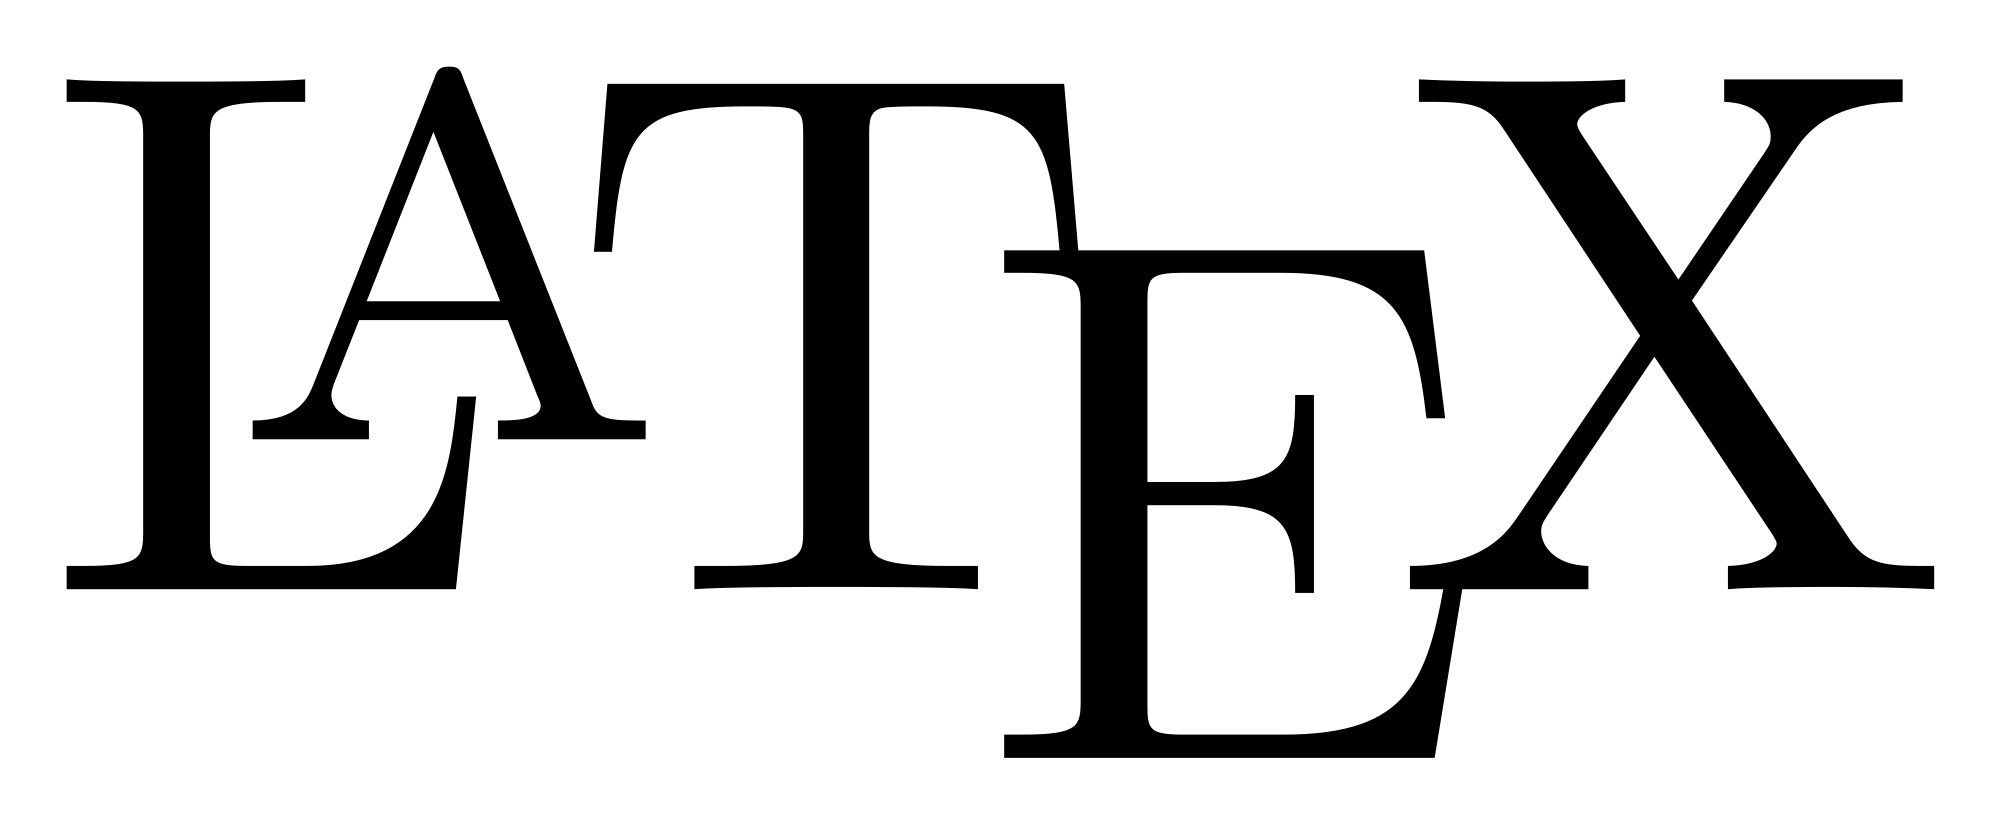
\includegraphics[width=4.5in]{images/latex.png}
    \caption{The \LaTeX\ logo.}
    \label{fig:latexlogo}
  \end{figure}
\end{frame}

I've already alluded to it as
an incredibly powerful software package, but at the end of the day,
\LaTeX\ is a \emph{document preparation system}.  In other words,
\LaTeX\ not only lets you type your document, but it also keeps track
of foot- and endnotes, bibliographies, cross-references, chapter and
section numbering, styles for section and subsection headings, and
much more.  It includes incredibly sophisticated algorithms for laying
out text on a page, advanced justification and autohyphenation
support, intelligent page breaking -- everything you would expect in a
serious piece of desktop publishing software.  And it does this
transparently, intelligently, and for free.

However, \LaTeX\ does not have a spell checker.  This is because --
and I cannot stress this enough -- \emph{\LaTeX\ is not a word
  processor!}  This is true in two senses: first, that \LaTeX\ does
not allow you to see the finished product as you are writing it

\begin{frame}
  \frametitle{What is \LaTeX?}
  \LaTeX\ is a sophisticated document preparation system and desktop
  publishing utility.
  \begin{block}{\LaTeX\ has \ldots}
    \begin{itemize}
    \item Footnotes and endnotes
    \item Bibliography support
    \item Reference tracking
    \item Stylistic uniformity
    \item Crazy algorithms
    \end{itemize}
  \end{block}
  \begin{block}{However \ldots}
    \begin{itemize}
    \item \emph{\LaTeX\ is not a word processor!}
    \end{itemize}
  \end{block}
\end{frame}

\begin{frame}
  \frametitle{What is \LaTeX\ not?}
  \LaTeX is a programming language, not a word processor.
  \begin{block}{\LaTeX\ will \emph{not} \ldots}
    \begin{itemize}
    \item Spell-check your documents
    \item Give you complete control over the way your document looks
    \item Let you see your document while you are writing it
    \end{itemize}
  \end{block}
  \begin{block}{Core \LaTeX\ philosophy:}
    You take care of writing; we'll take care of presentation.
    \begin{itemize}
    \item Humans write text.
    \item Computers figure out how to display the text.
    \end{itemize}
  \end{block}
\end{frame}

\subsection{Why should I use \LaTeX?}
\begin{frame}
  \frametitle{Why should I use \LaTeX?}
  Sometimes, presentation gets in the way of content.
  \begin{block}{Example: underlining vs.\ italics}
    \begin{itemize}
    \item Word processor way: set italics and/or underlining each time
    \item \LaTeX\ way: tell \LaTeX\ to \emph{emphasize}; set what that means later
    \end{itemize}
  \end{block}
  \begin{block}{Example: journal article / thesis}
    \begin{itemize}
    \item Word processor way: risk accidentally modifying provided template
    \item \LaTeX\ way: write your text, let \LaTeX\ worry about layout
    \end{itemize}
  \end{block}
\end{frame}

\begin{frame}
  \frametitle{Why should I not use \LaTeX?}
  \begin{itemize}
  \item Generally slower (exception: mathematics)
  \item Lack of complete control
  \end{itemize}
\end{frame}


\section{Your First \LaTeX\ Document}
\begin{frame}
  \frametitle{Your first \LaTeX\ document}
  \begin{block}{4 basic steps}
    \begin{enumerate}
    \item Write a .tex file using your favorite text editor
    \item Typeset using \LaTeX\ or \abbr{PDF}\LaTeX
    \item Preview the result using xdvi or xpdf (or Acrobat Reader or Evince)
    \item (optional) Convert the result to PostScript and print
    \end{enumerate}
  \end{block}
\end{frame}

% Steps to produce a document--15 min.
\subsection{Writing a .tex File}
\begin{frame}
  \frametitle{1. Write a .tex file}
  \begin{block}{hello.tex}
    \latexinput{code/hello.tex}
  \end{block}
\end{frame}

\subsection{Typesetting}
\begin{frame}
  \frametitle{2. Typeset using \LaTeX}
  \begin{block}{In a terminal:}
    \lstinputlisting{code/compiling.sh}
  \end{block}
\end{frame}

\begin{frame}
  \frametitle{2. Typeset using \LaTeX}
  \begin{block}{Result:}{\ttfamily\scriptsize
    This is pdfTeX, Version 3.1415926-1.40.10 (TeX Live 2009)\\
    entering extended mode\\
    (./hello.tex\\
    LaTeX2e <2009/09/24>\\
    Babel <v3.8l> and hyphenation patterns for english, usenglishmax, dumylang, noh\\
    yphenation, german-x-2009-06-19, ngerman-x-2009-06-19, ancientgreek, ibycus, ar\\
    abic, basque, bulgarian, catalan, pinyin, coptic, croatian, czech, danish, dutc\\
    h, esperanto, estonian, farsi, finnish, french, galician, german, ngerman, mono\\
    greek, greek, hungarian, icelandic, indonesian, interlingua, irish, italian, ku\\
    rmanji, latin, latvian, lithuanian, mongolian, mongolian2a, bokmal, nynorsk, po\\
    lish, portuguese, romanian, russian, sanskrit, serbian, slovak, slovenian, span\\
    ish, swedish, turkish, ukenglish, ukrainian, uppersorbian, welsh, loaded.\\
    (/usr/local/texlive/2009/texmf-dist/tex/latex/base/article.cls\\
    Document Class: article 2007/10/19 v1.4h Standard LaTeX document class\\
    (/usr/local/texlive/2009/texmf-dist/tex/latex/base/size10.clo))\\
    No file hello.aux.\\
    [1] (./hello.aux) )\\
    Output written on hello.dvi (1 page, 232 bytes).\\
    Transcript written on hello.log.}
  \end{block}
\end{frame}

\subsection{Previewing}
\begin{frame}
  \frametitle{3. Preview using xdvi}
  \begin{block}{New files!}
    \begin{itemize}
    \item hello.aux
    \item hello.dvi
    \item hello.log
    \end{itemize}
  \end{block}
  \begin{block}{hello.dvi}
    \lstinputlisting{code/previewing.sh}
  \end{block}
\end{frame}

\begin{frame}
  \frametitle{3. Preview using xdvi}
  \begin{block}{Result:}
    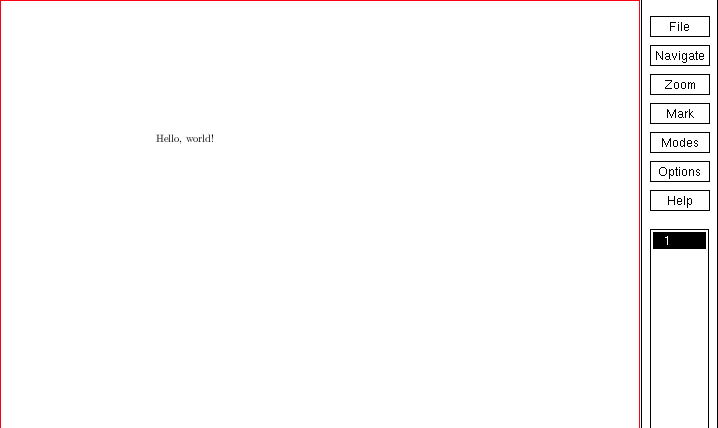
\includegraphics[width=4.5in]{images/xdvi.png}
  \end{block}
\end{frame}

\subsection{Printing}
\begin{frame}
  \frametitle{4. Convert to PostScript and print}
  \begin{block}{Converting to PostScript}
    \lstinputlisting{code/dvips.sh}
  \end{block}
  \begin{block}{Printing}
    \textbf{Don't run this command right now!}
    \lstinputlisting{code/lpr-athena.sh}
  \end{block}
\end{frame}


\subsection{When \LaTeX\ Complains}
\begin{frame}
  \frametitle{When \LaTeX\ complains}
  \begin{block}{Overfull/underfull hbox}
    \LaTeX\ couldn't make your text fit nicely on one line.
  \end{block}
  \begin{block}{Overfull/underfull vbox}
    \LaTeX\ couldn't make your text fit nicely on a page.
  \end{block}
  \begin{block}{Runaway argument}
    You forgot to close a brace.
  \end{block}
  \begin{block}{Solution}
    \begin{enumerate}
    \item Type x and hit enter
    \item Fix the error
    \item Re-run \LaTeX
    \end{enumerate}
  \end{block}
\end{frame}


\section{Basic Language Features}
\begin{frame}
  \frametitle{Sample document 1}
  ``Synthesizing Congestion Control Using Replicated Archetypes''

  Generated by SCIgen, the automatic computer science paper generator\\
  \url{pdos.csail.mit.edu/scigen/}
\end{frame}

\subsection{Commands}
\begin{frame}
  \frametitle{Declarations and environments}
  \begin{block}{Declarations \ldots}
    \begin{itemize}
    \item Are stated once
    \item Take effect until further notice
    \item Can be constrained using curly braces
    \end{itemize}
    Example: $\backslash$documentclass
  \end{block}
  \begin{block}{Environments \ldots}
    \begin{itemize}
    \item Have corresponding $\backslash$begin and $\backslash$end declarations
    \item Apply formatting to their contents
    \end{itemize}
    Example: $\backslash$begin\{document\} / $\backslash$end\{document\}
  \end{block}
\end{frame}

\subsection{$\backslash$documentclass}
\begin{frame}
  \frametitle{The $\backslash$documentclass declaration}
  $\backslash$documentclass tells \LaTeX\ what basic document template
  to use.
  \begin{block}{Other templates (``classes''):}
    \begin{itemize}
    \item book
    \item report
    \item letter
    \item revtex4-1
    \item thesis
    \item beamer
    \end{itemize}
  \end{block}
\end{frame}

\subsection{Structure}
\begin{frame}
  \frametitle{Sectioning declarations}
  \begin{itemize}
  \item $\backslash$part (book only)
  \item $\backslash$chapter (book and report only)
  \item $\backslash$section
  \item $\backslash$subsection
  \item $\backslash$subsubsection
  \item $\backslash$paragraph
  \item $\backslash$subparagraph
  \item $\backslash$subsubparagraph
  \end{itemize}
  Example: $\backslash$chapter\{A Mad Tea-Party\}
\end{frame}

\subsection{Command Arguments}
\begin{frame}
  \frametitle{Arguments}
  Arguments can be required or optional.
  \begin{block}{Required arguments \ldots}
    \begin{itemize}
    \item Are placed in curly braces
    \item Cause \LaTeX\ to complain if left out
    \end{itemize}
    Example: $\backslash$documentclass\{\textbf{article}\}
  \end{block}
  \begin{block}{Optional arguments \ldots}
    \begin{itemize}
    \item Are placed in square brackets
    \item Don't cause errors if left out
    \item Come before required arguments
    \end{itemize}
    Example: $\backslash$documentclass[\textbf{12pt,letterpaper}]\{article\}
  \end{block}
\end{frame}

\subsection{Document components}
\begin{frame}
  \frametitle{The title}
  \begin{block}{Place in preamble (before $\backslash$begin\{document\}):}
    $\backslash$title\{Synthesizing Congestion Control Using Replicated Archetypes\}\\
    $\backslash$author\{Benjamin Barenblat$\backslash$$\backslash$MIT $\backslash$and SCIgen$\backslash$$\backslash$CSAIL\}\\
    $\backslash$date\{$\backslash$today\}
  \end{block}
  \begin{block}{Place in document:}
    $\backslash$maketitle
  \end{block}
  Some classes allow for more preamble commands.
\end{frame}

\begin{frame}
  \frametitle{Including graphics}
  Straight \LaTeX\ requires documents to be in encapsulated PostScript format.
  \begin{block}{Place in preamble:}
    $\backslash$usepackage\{graphicx\}
  \end{block}
  \begin{block}{Place in document:}
    $\backslash$begin\{figure\}\\
    \quad$\backslash$begin\{center\}\\
    \qquad$\backslash$includegraphics\{doc1/flowchart.eps\}\\
    \quad$\backslash$end\{center\}\\
    \quad$\backslash$caption\{The diagram used by Oxymel.\}\\
    $\backslash$end\{figure\}
  \end{block}
\end{frame}

\begin{frame}
  \frametitle{Labeling figures}
  \begin{block}{Place after caption:}
    $\backslash$label\{robots\}
  \end{block}
  \begin{block}{Place in appropriate location:}
    \ldots\ figure$\sim$$\backslash$ref\{robots\}
  \end{block}
  You will have to run \LaTeX\ twice!
\end{frame}

\begin{frame}
  \frametitle{Labeling figures and stuff}
  \begin{block}{Place after appropriate command:}
    $\backslash$label\{robots\}
  \end{block}
  \begin{block}{Place in appropriate location:}
    \ldots\ $\backslash$ref\{robots\}
  \end{block}
  You will have to run \LaTeX\ twice!
\end{frame}

\begin{frame}
  \frametitle{Tables}
  \begin{block}{Recall figures:}
    $\backslash$begin\{figure\}\\
    \quad$\backslash$begin\{center\}\\
    \qquad$\backslash$includegraphics\{doc1/flowchart.eps\}\\
    \quad$\backslash$end\{center\}\\
    \quad$\backslash$caption\{The diagram used by Oxymel.\}\\
    $\backslash$end\{figure\}
  \end{block}
  \begin{block}{Similar method for tables:}
    $\backslash$begin\{table\}\\
    \quad$\backslash$begin\{center\}\\
    \qquad$\backslash$includegraphics\{doc1/datatable.eps\}\\
    \quad$\backslash$end\{center\}\\
    \quad$\backslash$caption\{Our raw data.\}\\
    $\backslash$end\{table\}
  \end{block}
\end{frame}

\begin{frame}
  \frametitle{Tabular}
  \begin{block}{Code:}
    $\backslash$begin\{tabular\}\{\ell\ \ell\ \ell\}\\
      \quad Language \& Seek time \& Write time$\backslash$$\backslash$\\
      \quad$\backslash$hline\\
      \quad BLooP \& 27 \& 42$\backslash$$\backslash$\\
      \quad FLooP \& 12 \& 19$\backslash$$\backslash$\\
      \quad GLooP \& 11 \& 22\\
    $\backslash$end\{tabular\}
  \end{block}
  \begin{block}{Result:}
    \begin{tabular}{l l l}
      Language & Seek time & Write time\\
      \hline
      BLooP & 27 & 42\\
      FLooP & 12 & 19\\
      GLooP & 11 & 22
    \end{tabular}
  \end{block}
\end{frame}

\begin{frame}
  \frametitle{Lists}
  Lists can be numbered (enumerated) or bulleted (itemized).
  \begin{block}{Numbered lists:}
    $\backslash$begin\{enumerate\}\\
    \quad$\backslash$item Item 1\\
    \quad$\backslash$item Item 2\\
    $\backslash$end\{enumerate\}
  \end{block}
  \begin{block}{Bulleted lists:}
    $\backslash$begin\{itemize\}\\
    \quad$\backslash$item Item 1\\
    \quad$\backslash$item Item 2\\
    $\backslash$end\{itemize\}
  \end{block}
\end{frame}

\begin{frame}
  \frametitle{Quoting other works}
  \begin{block}{quote}
    \small$\backslash$begin\{quote\}\\
    \quad Here's a single-paragraph quote.\\
    $\backslash$end\{quote\}\normalsize
  \end{block}
  \begin{block}{quotation}
    \small$\backslash$begin\{quotation\}\\
    \quad Here's a multiparagraph quote.\\
    \\
    \quad Here's the second paragraph.\\
    $\backslash$end\{quotation\}\normalsize
  \end{block}
  \begin{block}{verse}
    \small$\backslash$begin\{verse\}\\
    \quad Here's some poetry.$\backslash\backslash$\\
    \quad Here's the second line.$\backslash\backslash$\\
    $\backslash$end\{verse\}\normalsize
  \end{block}
\end{frame}

\begin{frame}
  \frametitle{Finishing touches}
  \begin{block}{The abstract:}
    $\backslash$begin\{abstract\}\\
    \quad Yada yada yada\ldots.\\
    $\backslash$end\{abstract\}
  \end{block}
  \begin{block}{A title page}
    $\backslash$documentclass[\textbf{titlepage}]\{article\}
  \end{block}
  \begin{block}{Real headers}
    $\backslash$pagestyle\{headings\}
  \end{block}
\end{frame}

\begin{frame}
  \frametitle{Miscellaneous}
  \begin{block}{Spaces}
    \begin{tabular}{l l}
      $\sim$ & nonbreaking space\\
      $\backslash$\ \null & force normal interword space\\
      & \quad(e.g., \texttt{Steele et al.$\backslash$ discovered})\\
      $\backslash$\url{@}. & force end-of-sentence space\\
      & \quad(e.g., \texttt{I program in C$\backslash$\url{@}\@. You?})\\
      $\backslash$hspace\{1in\} & make horizontal space\\
      $\backslash$vspace\{1in\} & make vertical space
    \end{tabular}
  \end{block}
  \begin{block}{Breaking}
    \begin{tabular}{l l}
      $\backslash\backslash$ & force new line\\
      $\backslash$newpage & force new page\\
      $\backslash$noindent & force no indentation of current paragraph
    \end{tabular}
  \end{block}
  Comments: Anything after \% on a single line is ignored.
\end{frame}


\subsection{Customizing \LaTeX}
\begin{frame}
  \frametitle{Customizing \LaTeX}
  Some customization commands are built-in.
  \begin{block}{Changing font face:}
    $\backslash$emph\{\emph{text}\},
    $\backslash$textnormal\{\textnormal{text}\},
    $\backslash$textrm\{\textrm{text}\},
    $\backslash$textsf\{\textsf{text}\},
    $\backslash$texttt\{\texttt{text}\},
    $\backslash$textbf\{\textbf{text}\},
    $\backslash$textit\{\textit{text}\},
    $\backslash$textsc\{\textsc{text}\}
  \end{block}
  \begin{block}{Changing font size:}
    \tiny$\backslash$tiny\normalsize,
    \scriptsize$\backslash$scriptsize\normalsize,
    \footnotesize$\backslash$footnotesize\normalsize,
    \small$\backslash$small\normalsize,
    \normalsize$\backslash$normalsize\normalsize,
    \large$\backslash$large\normalsize,
    \Large$\backslash$Large\normalsize,
    \LARGE$\backslash$LARGE\normalsize,
    \huge$\backslash$huge\normalsize,
    \Huge$\backslash$Huge\normalsize
  \end{block}
  \begin{block}{Changing alignment:}
    $\backslash$begin\{center\},
    $\backslash$begin\{flushright\},
    $\backslash$begin\{flushleft\}
  \end{block}
\end{frame}

\begin{frame}
  \frametitle{Customizing \LaTeX}
  Customizations can also occur through \emph{packages}.
  \begin{block}{Including a package:}
    $\backslash$usepackage\{packagename\}
  \end{block}
  \begin{block}{Useful packages}
    graphicx, geometry, setspace, fancyhdr, calc, mathpazo, microtype,
    amsmath, amsfonts, amsthm, amssymb, url, ulem, textcomp, listings,
    eco, mathtools, mhchem, units, wrapfig, color, ccaption, titlesec,
    epstopdf, tabularx, tocloft \ldots
  \end{block}
\end{frame}

\begin{frame}
  \frametitle{A survey of useful packages}
  \begin{block}{geometry}
    Controls margins:\\
    \quad$\backslash$usepackage[margin=1.1in]\{geometry\}
  \end{block}
  \begin{block}{setspace}
    Allows you to use double and 1.5 spacing:\\
    \quad$\backslash$usepackage\{setspace\}\\
    \quad$\backslash$doublespacing
  \end{block}
  \begin{block}{fancyhdr}
    Controls header and footer:\\
    \small\quad$\backslash$usepackage\{fancyhdr\}\\
    \quad$\backslash$pagestyle\{fancy\}\\
    \quad$\backslash$fancyhf\{\} \% Reset header and footer\\
    \quad$\backslash$fancyhead[R]\{$\backslash$thepage\} \% This puts the page in the right of the header
  \end{block}
\end{frame}

\begin{frame}
  \frametitle{Changing fonts}
  Fonts are usually loaded through packages as well.
  \begin{tabular}{l l}
    $\backslash$usepackage[urw-garamond]\{mathdesign\} & Garamond\\
    $\backslash$usepackage\{mathpazo\} & Palatino\\
    $\backslash$usepackage[scaled]\{helvet\} & Helvetica\\
    $\backslash$usepackage\{courier\} & Courier\\
    $\backslash$renewcommand*$\backslash$sfdefault\{uop\} & Optima\\
    $\backslash$usepackage\{concrete\} & Computer Concrete\\
    $\backslash$usepackage\{tgbonum\} & Bookman\\
    $\backslash$usepackage\{txfonts\} & Times
  \end{tabular}

  More fonts are available at The \LaTeX\ Font Catalogue,
  \url{www.tug.dk/FontCatalogue/}.
\end{frame}


\section{Mathematics}
\begin{frame}
  \frametitle{Typesetting mathematics}
  \LaTeX's math support far outstrips that of any other available
  piece of software.
  \begin{block}{The Leibniz integral rule}
    \begin{align*}
      \frac{d}{d\alpha} \int_{a(\alpha)}^{b(\alpha)} f(x,\alpha) dx &= \frac{db(\alpha)}{d\alpha} f\big(b(\alpha), \alpha\big) - \frac{da(\alpha)}{d\alpha}f\big(a(\alpha),\alpha\big)\\ &\quad + \int_{a(\alpha)}^{b(\alpha)} \frac{\partial}{\partial\alpha} f(x,\alpha) dx
    \end{align*}
  \end{block}
  \begin{block}{Generalized Stokes theorem}
    If $\omega$ is an $(n-1)$-form with compact support on $M$ and
    $\partial M$ denotes the boundary of $M$ with its induced
    orientation, then
    \begin{equation*}
      \int_M \text{d}\omega = \oint_{\partial M} \omega.
    \end{equation*}
  \end{block}
\end{frame}

\subsection{Math Mode}
\begin{frame}
  \frametitle{Text and math modes}
  \LaTeX\ is always operating in either text mode, display math mode,
  or inline math mode.
  \begin{block}{Inline math mode}
    \begin{itemize}
    \item Enter/exit using \$\ldots\$ or $\backslash$(\ldots$\backslash$)
    \item Large symbols and super/subscripts are squashed:
    \end{itemize}
    \begin{center}\vspace{-0.5em}$\int_1^\infty e^-x dx$\qquad$\sum_{n=0}^\infty n!$\qquad$\big[\begin{smallmatrix}1 & 0 \\ 0 & 1\end{smallmatrix}\big]$\end{center}
  \end{block}
  \begin{block}{Display math mode}
    \begin{itemize}
    \item Enter/exit using $\backslash$begin\{equation\}\ldots$\backslash$end\{equation\} or $\backslash$[\ldots$\backslash$]
    \item Large symbols and super/subscripts are displayed in full glory
    \item Equations can be numbered
    \end{itemize}
    \[\int_1^\infty e^-x dx\qquad\sum_{n=0}^\infty n!\qquad\begin{bmatrix}1 & 0 \\ 0 & 1\end{bmatrix}\]
  \end{block}
\end{frame}

\subsection{Basic mathematics}
\begin{frame}
  \frametitle{Basic mathematics}
  The vast majority of math commands are highly logical.

  \begin{tabular}{r l r l}
    $974$ & 974 & $x$ & x\\
    $4 + 2$ & 4 + 2 & $49 \pm 71$ & 49 $\backslash$pm 71\\
    $\sqrt[3]{5}$ & $\backslash$sqrt[3]\{5\} & $\phi \in U$ & $\backslash$phi $\backslash$in U\\
    $x_1^2$ & x\_1\^{}2 & $f''(\xi)$ & f$''$($\backslash$xi)\\
    $\frac{x}{y}$ & $\backslash$frac\{x\}\{y\} & $\forall x\exists y$ & $\backslash$forall x$\backslash$exists y\\
    $\sum_{k=1}^{n} k$ & $\backslash$sum\_\{k=1\}\^{}n k & $U \cap V$ & U$\backslash$cap V\\
    $x \leqslant y$ & x $\backslash$leqslant y & $P \Leftrightarrow Q$ & P$\backslash$Leftrightarrow Q\\
    $2 \ne 4$ & 2 $\backslash$ne 4 & $\mathbb{R} \subset \mathbb{C}$ & $\backslash$mathbb\{R\}$\backslash$subset\\
    $\nabla \cdot \mathbf{\Psi}$ & $\backslash$nabla$\backslash$cdot$\backslash$mathbf\{$\backslash$Psi\} && $\backslash$mathbb\{C\}\\
    $\hat{\i}\times\hat{\j}=\hat{\mathsf{k}}$ & \multicolumn{3}{l}{$\backslash$hat\{$\backslash$i\}$\backslash$times$\backslash$hat\{$\backslash$j\}=$\backslash$hat\{$\backslash$k\}}\\
  \end{tabular}

  Detexify$^2$ (\url{detexify.kirelabs.org/}) gives commands for
  any symbol.
\end{frame}

\subsection{Environments}
\begin{frame}
  \frametitle{Mathematics packages and environments}
  \begin{itemize}
  \item Use $\backslash$usepackage\{amsfonts,amsmath,amssymb,amsthm\}
    unless you have a good reason not to.
  \item $\backslash$usepackage\{esint\} will get you cool integral signs.
  \end{itemize}
  \begin{block}{equation}
    \begin{equation}
      \label{gaussthm}
      \oiint_{\partial\Omega}\mathbf{F}\cdot d\mathbf{S} = \iiint_\Omega\nabla\cdot\mathbf{F}dxdydz
    \end{equation}
  \end{block}
  \begin{block}{equation*}
    \begin{equation*}
      \oiint_{\partial\Omega}\mathbf{F}\cdot d\mathbf{S} = \iiint_\Omega\nabla\cdot\mathbf{F}dxdydz
    \end{equation*}
  \end{block}
  {\small The Short Math Guide for
  \LaTeX\ (\url{ftp://ftp.ams.org/pub/tex/doc/amsmath/short-math-guide.pdf}) has a
  full listing.}
\end{frame}

\begin{frame}
  \frametitle{Mathematics packages and environments}
  \begin{block}{align}
    \latexinput{code/align.tex}
    \begin{align}
      a &= \oiint_{\partial\Omega}\mathbf{F}\cdot d\mathbf{S}  &  (3)(5 + 7) &= (3)(12)\\
        &= \iiint_\Omega\nabla\cdot\mathbf{F}dxdydz  &  &= 36
    \end{align}
  \end{block}
\end{frame}

\begin{frame}
  \frametitle{Labeling figures and stuff}
  \begin{block}{Place after appropriate command:}
    $\backslash$label\{robots\}
  \end{block}
  \begin{block}{Place in appropriate location:}
    \ldots\ $\backslash$ref\{robots\}
  \end{block}
  You will have to run \LaTeX\ twice!
\end{frame}
\begin{frame}
  \frametitle{Labeling figures and equations and stuff \ldots}
  \begin{block}{Place in environment:}
    $\backslash$label\{gaussthm\}
  \end{block}
  \begin{block}{Place in appropriate location:}
    \ldots\ equation~$\backslash$ref\{gaussthm\}
  \end{block}
  You will have to run \LaTeX\ twice!
\end{frame}


\section{Specialized Applications}
\subsection{Beamer}
\begin{frame}
  \frametitle{Presentations with Beamer}
  \begin{block}{Why use Beamer?}
    \begin{itemize}
    \item Just as full-featured as PowerPoint, OpenOffice.org Impress, etc.
    \item Easy to get going (it's \LaTeX!)
    \item Variety of predefined themes for professional presentations
    \item Math support
    \end{itemize}
  \end{block}
  \begin{block}{Getting started}
    \begin{itemize}
    \item $\backslash$documentclass\{beamer\}
    \item frame environment
    \end{itemize}
  \end{block}
\end{frame}

\begin{frame}
  \frametitle{New commands}
  \begin{block}{Preamble}
    \begin{itemize}
    \item $\backslash$documentclass\{beamer\}
    \item $\backslash$usetheme\{CambridgeUS\} sets theme
    \item $\backslash$institute\{CSAIL$\backslash\backslash$\mit\} appears below author name
    \end{itemize}
  \end{block}
  \begin{block}{Document body}
    \begin{itemize}
    \item frame environment
      \begin{itemize}
      \item $\backslash$frametitle\{\}
      \item block environment
      \end{itemize}
    \item $\backslash$titlepage makes a title slide ($\backslash$maketitle is for handouts)
    \item $\backslash$tableofcontents makes an outline slide
    \item $\backslash$section, $\backslash$subsection diminish in importance
    \end{itemize}
  \end{block}
\end{frame}


\section{Where to Go from Here}
\begin{frame}
  \frametitle{Where to go from here}
  {\small
  \begin{block}{Further resources}
    \begin{itemize}
    \item \emph{The Not So Short Introduction to \LaTeX\ 2}$_\varepsilon$:\\
      \url{www.ctan.org/tex-archive/info/lshort/english/lshort.pdf}
    \item The \LaTeX\ 2$_\varepsilon$ cheat sheet:\\
      \url{www.stdout.org/~winston/latex/latexsheet.pdf}
    \item \emph{A Short Math Guide for \LaTeX}:\\
      \url{ftp://ftp.ams.org/pub/tex/doc/amsmath/short-math-guide.pdf}
    \item The \texttt{texdoc} command
    \end{itemize}
  \end{block}
  }
  \begin{block}{\LaTeX\ on your own computer}
    \begin{itemize}
    \item Linux: \TeX\ Live (use your package manager)
    \item Mac OS: Mac\TeX: \url{www.tug.org/mactex/}
    \item Windows: Mik\TeX: \url{www.miktex.org/}
    \end{itemize}
  \end{block}
\end{frame}
\end{document}
